	\documentclass[twoside]{article}
\usepackage{../../estilo-ejercicios}
\renewcommand{\baselinestretch}{1,3}
%--------------------------------------------------------
\begin{document}

\title{Ejercicios de Topología Algebraica}
\author{Javier Aguilar Martín}
\maketitle

\begin{ejercicio}{2.2.36}
Probar que $H_i(X\times S^n)\cong H_i(X)\oplus H_{i-n}(X)$ para todo $i$ y $n$, donde $H_i=0$ para $i<0$. Esto es, probar que $H_i(X\times S^n)=H_i(X)\oplus H_i(X\times S^n,X\times\{x_0\})$ y $H_i(X\times S^n,X\times\{x_0\})\cong H_{i-1}(X\times S^{n-1},X\times\{x_0\})$.
\end{ejercicio}
\begin{solucion}
Probamos primero el último isomorfismo usando la sucesión relativa de Mayer-Vietoris. Para ello descomponemos $X\times S^n$ usando la descomposición de $S^n$ en dos $U$ y $V$ mitades contráctiles con $U\cap V\simeq S^{n-1}$. Tenemos entonces que $X\times U\simeq X\times V\simeq X\times \{x_0\}\cong X$. Como $H_i(X,X)=0$ para todo $i$ y $X$, y $(X\times U)\cap (X\times V)=X\times (U\cap V)\simeq X\times S^{n-1}$,  la sucesión relativa de Mayer-Vietoris nos da el isomorfismo $H_i(X\times S^n,X\times\{x_0\})\cong H_{i-1}(X\times S^{n-1},X\times\{x_0\})$. 

Observamos ahora que $X\times\{x_0\}$ es un retracto de $X\times S^n$ mediante la retración $r(x,y)=(x,x_0)$, que claramente verifica $r\circ i=Id$. En homología (y en complejos de cadenas) se induce por tanto $r_*\circ i_*=Id$, de donde deducimos que $i_*:H_i(X\times\{x_0\})\to H_i(X\times S^n)$ es inyectiva y además tiene una sección $r_*$, por lo que la sucesión exacta inducida por $0\to C_*(X\times\{x_0\})\xrightarrow{i_*} C_*(X\times S^n)\to C_*(X\times S^n,X\times\{x_0\})\to 0$ en homología
\[
0\to H_i(X\times\{x_0\})\to H_i(X\times S^n)\to H_i(X\times S^n,X\times\{x_0\})\to 0
\]
escinde (los ceros provienen de la sucesión exacta larga del par aplicando que $i_*$ es inyectiva). Esto es, $$H_i(X\times S^n)\cong  H_i(X\times\{x_0\})\oplus H_i(X\times S^n,X\times\{x_0\})\cong H_i(X)\oplus H_i(X\times S^n,X\times\{x_0\}).$$

Ahora, aplicamos $n$ veces el isomorfismo $H_i(X\times S^n,X\times\{x_0\})\cong H_{i-1}(X\times S^{n-1},X\times\{x_0\})$, que nos da $H_i(X\times S^n,X\times\{x_0\})\cong H_{i-n}(X\times S^0,X\times\{x_0\})$. Como $X\times S^0\cong X\sqcup X$ y $X\times \{x_0\}\cong X$, tenemos que el complejo de cadenas $C_*(X\times S^0,X\times\{x_0\})$ es isomorfo a $C_*(X)$ y por tanto también lo es su homología, esto es, $H_i(X\times S^n,X\times\{x_0\})\cong H_{i-n}(X)$, con lo que combinando los resultados obtenidos deducimos finalmente
$
H_i(X\times S^n)\cong H_i(X)\oplus H_{i-n}(X).
$

%\url{https://math.stackexchange.com/questions/669600/hatcher-problem-2-2-36}
\end{solucion}

\newpage

\begin{ejercicio}{}
Dar un ejemplo de aplicación $f:S^n\to S^n$ con $n>0$ tal que para todo $y\in S^{n}$, $f^{-1}(y)$ consta de una cantidad infinita de puntos. 
\end{ejercicio}
\begin{solucion}

\end{solucion}

\newpage


%\begin{ejercicio}{de las naranjas}
%Para el espacio $X$ de la imagen (donde las esferas se consideran huecas), calcular la homología local de todos sus puntos, hallar la mayor cantidad posible de subespacios $A\subseteq X$ tales que cualquier homeomorfismo $f:A\to X$ satisfaga $f(A)\subseteq A$, y estudiar si es posible asegurar que alguna potencia $f^n$ tenga puntos fijos, y en su caso cuántos. 
%
%\begin{figure}[h!]
%\centering
%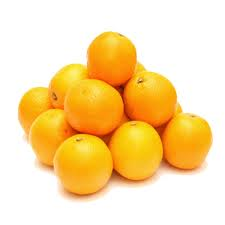
\includegraphics[scale=0.5]{naranjas}
%\end{figure}
%\end{ejercicio}
%\begin{solucion}
%Topológicamente distinguimos dos tipos de puntos en el espacio $X$: los puntos que tienen entornos homeomorfos a un disco abierto y los puntos donde las esferas se pegan, que tienen entornos homeomorfos a la unión puntual de dos discos abiertos. Sea $x\in X$ un punto del primer tipo y sea $U$ un entorno homeomorfo a un disco abierto. Entonces $U-x\simeq S^1$. La versión reducida de la sucesión exacta larga de homología relativa nos da $H_*(U,U-x)\cong \widetilde{H}_*(S^1)$, por lo que es 0 en todos los grados salvo $H_1(U,U-x)\cong\Z$. Sea ahora $x\in X$ con un entorno de $U$ de $x$ homeomorfo a la unión puntual de dos discos abiertos, de modo que $U-x\simeq S^1\sqcup S^1$. La sucesión exacta larga de homología relativa nos da $H_i(U,U-x)=0$ para $i>2$, $H_2(U,U-x)=\Z\oplus\Z$. Para los grados más bajos usamos la versión reducida, la cual nos da $H_1(U,U-x)=\Z$ y $H_0(U,U-x)=0$. Alternativamente podemos calcular la homología en grado 1 usando el ejercicio 2.1.16, de modo que $H_0(U,U-x)=0$ porque $U-x$ corta a la única componente conexa de de $U$. Como vemos, los puntos del primer tipo tienen homología local distinta a los del segundo, pues en el primer caso $H_2(U,U-x)=0$ y en el segundo $H_2(U,U-x)=\Z\oplus\Z$.
%
%\vspace{0.5cm}
%
%Vamos a la segunda parte del ejercicio. A los puntos del primer tipo los llamamos puntos de tipo I y a los del segundo tipo los llamamos puntos de tipo II. Lo primero que debemos notar es que cualquier homeomorfismo es en particular homeomorfismo local, y por tanto preserva la homología local, por lo que llevará puntos de tipo I en puntos de tipo I y puntos de tipo II en puntos de tipo II (todo esto en $A$, un punto de tipo $I$ en $A$ puede ser de tipo II en $X$). Vamos a suponer $A\neq\emptyset$, ya que en este caso trivialmente $f(A)=A$ y no hay puntos fijos para $f$ ni ninguna de sus potencias. Vamos a tratar primero el siguiente caso por orden de trivialidad, que sería $A=X$, donde también $f(A)=A$. Además, como hay una cantidad finitas de puntos de tipo II, digamos $k$ por ahorrarnos contar la cantidad exacta de este ejemplo, $f$ induce una permutación $\sigma_f\in S_k$, luego para $n=o(\sigma_f)$, $f^n$ tiene al menos $k$ puntos fijos. Para una potencia menor no es posible asegurar el mínimo de puntos fijos puesto que dependerá de la permutación en concreto, y tampoco podemos asegurar que no haya más porque podría haber puntos fijos en el resto de $X$. Una vez encontremos otro subespacio $A$ con $f(A)=A$, el mismo razonamiento será válido.
%
%%En primer lugar, $A$ no puede ser una esfera completa porque no tendría puntos de tipo II pero cualquier homeomorfismo la llevaría a una de las esfera, que sí tienen puntos de tipo II en $X$. Por otro lado, si $A$ está estrictamente contenido en una esfera menos los puntos de tipo II, siempre podemos tomar un homeomorfismo que deforme $A$ de modo que puntos que no estaban en $A$ aparezcan en la imagen. Así que $A$ debería contener como componentes conexas a algunas esferas menos sus puntos de tipo II. Observemos que las esferas del primer nivel tienen 3 puntos de tipo II salvo la central que tiene 4, las del segundo nivel tienen 5 puntos de tipo II y la esfera del tercer nivel tiene 4 puntos de tipo II. Por tanto, las componentes conexas de un nivel de $A$ van en ese mismo nivel, pues las de distintos niveles no son homeomorfas, pero las de un mismo nivel sí lo son. Si hubiera un nivel en el que $A$ tuviera alguna componente conxa pero no todas, entonces un homeomorfismo podría enviar una de las componentes conexas de $A$ en una de las de ese mismo nivel que no está en $A$. Por tanto, para cada nivel, $A$ debe o bien contenerlo por completo o bien no contener nada. Esto nos da todas las posibilidades para el caso en el que $A$ no contenga puntos de tipo II. 
%
%Si $A$ está estrictamente contenido en una de las esferas, podemos elegir un homeomorfismo que deforme $A$ de modo que puntos que no estaban en $A$ aparezcan en la imagen, así que $A$ debe contener esferas completas y solo esferas completas. De hecho debe contener más de una, porque si contuviera solo una, podría ser enviada con un homeomorfismo a cualquiera de las otra. De esto además se deduce que si $f(A)\subseteq A$, entonces se da de hecho la igualdad, ya que los homeomorfismos se reducen a permutaciones de esferas que mantienen la homología local y el razonamiento de los puntos fijos será valido para todos los subespacios fijos que encontremos.
%
%%Supongamos que $A\neq\emptyset$ EN ESTE PÁRRAFO LA CANTIDAD DE PUNTOS DE TIPO II ESTÁ MAL está contenido en el primer nivel de la pirámide. Entonces debe contener todas las esferas que dan al exterior, de lo contrario un homeomorfismo podría llevar una de las esferas de $A$ que dan al exterior a una de las que dan al exterior que no están en $A$. Esto es independiente de si $A$ contiene la esfera central porque cualesquiera combinaciones de la esfera central con $m$ de las que dan al exterior son homeomorfas entre sí. Además podemos comprobar que de hecho es necesario que en este caso $A$ contenga a la esfera central, de lo contrario podríamos elegir un homeomorfismo que llevara 3 esferas que hagan esquina en dos del segundo nivel y la del tercero. La esfera central tiene 4 puntos de tipo II, luego un homeomorfismo que no la lleve en sí misma solo podría llevarla a la esfera superior (en principio podría llevarla al segundo nivel, ocupando solo 4 de las 5 esferas adyacentes, pero se comprueba por inspección que esto no da lugar a un homeomorfismo) junto con las 4 esferas con las que está en contacto, que ocuparían el segundo nivel, pero esto no da posibilidad para que el resto de esferas de $A$ puedan ser mapeadas con un homeomorfismo, así que la esfera central debe quedar fija. 
%De ahora en adelante usaremos la siguiente notación para facilitar el enunciado y la comprensión: a la esfera superior la denotamos $S$, a la esfera central del nivel inferior la denotamos $C$, al resto de esferas del primer nivel las denotamos $E_i$, $i=1,\dots, 8$, siendo impares en las esquinas, y a las esferas del segundo nivel las denotamos $Z_j$, $j=1,\dots, 4$.
%
%
%Empecemos considerando subespacios que contentan a $S$. Es claro que añadiendo esferas solo del segundo nivel siempre podemos encontrar otros subespacios homeomorfos. Además, si incluimos alguna $Z_j$ en $A$, tendremos que incluirlas todas por simetría. Si además añadimos la esfera $C$, entonces ya no hay otro subespacio en el que haya dos esferas con 4 puntos de tipo II así que este verifica $f(A)=A$ para todo homeomorfismo. Además podríamos seguir añadiendo o bien las $E_{2k}$ o bien las $E_{2k+1}$ (o todas, pero eso nos daría $X$, que ya lo hemos estudiado). 
%
%Si no añadimos la esfera central, podemos o bien añadir las esferas $E_{2k}$ o bien las $E_{2k+1}$ (o todas). En cualquier otro caso podríamos encontrar un homeomorfismo que no deje invariante $A$ mediante rotaciones y simetrías. En los casos que hemos dado como válidos, $f(A)=A$ para cualquier homeomorfismo, ya que cualquier esfera que se enviara a una que no hayamos incluido tendría una cantidad distinta de puntos de tipo II. 
%
% Dentro de los subespacios que contienen a la esfera $S$ faltarían aquellos que no tienen ninguna esfera $Z_j$. Es claro que si $A$ no contiene la esfera $C$, entonces debe contener todas las exteriores y que este este sería un espacio invariante. Si $A$ contiene a $C$ hay más posibilidades. Una de ellas es que tenga todas las $E_i$, pero también podemos quedarnos solo con las $E_{2k}$ o solo con las $E_{2k+1}$, siendo esta última la única forma de elegir 6 esferas aisladas. 
% 
% Analizamos ahora los subespacio que no contienen a $S$. Si no $A$ no contiene tampoco ninguna $Z_j$, surgen los subespacios invariantes siguientes: $\bigcup_{i=0}^8E_i$ y $C\cup \bigcup_{k=0}^4E_{2k}$. En cualquier otro caso podríamos enviar homeomórficamente esferas de $A$ a un nivel superior o a esferas del nivel inferior que no estén en $A$. 
%
% 
% Si $A$ contiene alguna $Z_j$ pero no todas, por simetría podemos encontrar subespacios homeomorfos a $A$ que tienen esferas en este nivel que no están en $A$. Por tanto, nos centramos en los subespacios que contienen a todas las $Z_j$, que además deben contener esferas del nivel inferior, ya que hay más subespacios homeomorfos al espacio $\bigcup_{j=1}^4Z_j$. Si contiene además a $C$, tendrá que contener alguna esfera más porque de lo contrario podría enviarse $C\to S$. Por simetría, es necesario además que como mínimo sean o las cuatro $E_{2k}$ o las cuatro $E_{2k+1}$ (o todas las $E_i$). Si $A$ no contiene a $C$ en realidad también encontramos exactamente las mismas posibilidades, así que con esto hemos analizado todos los casos posibles. 
% 
%
% 
%\end{solucion}

\end{document}
